\chapter{Alignment performance at high laser power}
\section{Beam spot motion}
\begin{itemize} 
\item calibration
\item residuals, perhaps for different kinds of seismic
\end{itemize}

\section{Angular mirror motion}
When the gain is really high, comparing the calibrated error and
control signals shows just what the control loop is doing. The error
is the residual and the control is what there would be without the
loop.

error * (1+G) is the motion without the loop, where G is the open loop gain.

\begin{itemize} 
\item optical lever calibration
\item residuals, perhaps for different kinds of seismic
\item compare to mirror motion with no ifo (demonstrate ASC suppression)
\end{itemize}


\begin{figure}
\begin{centering}
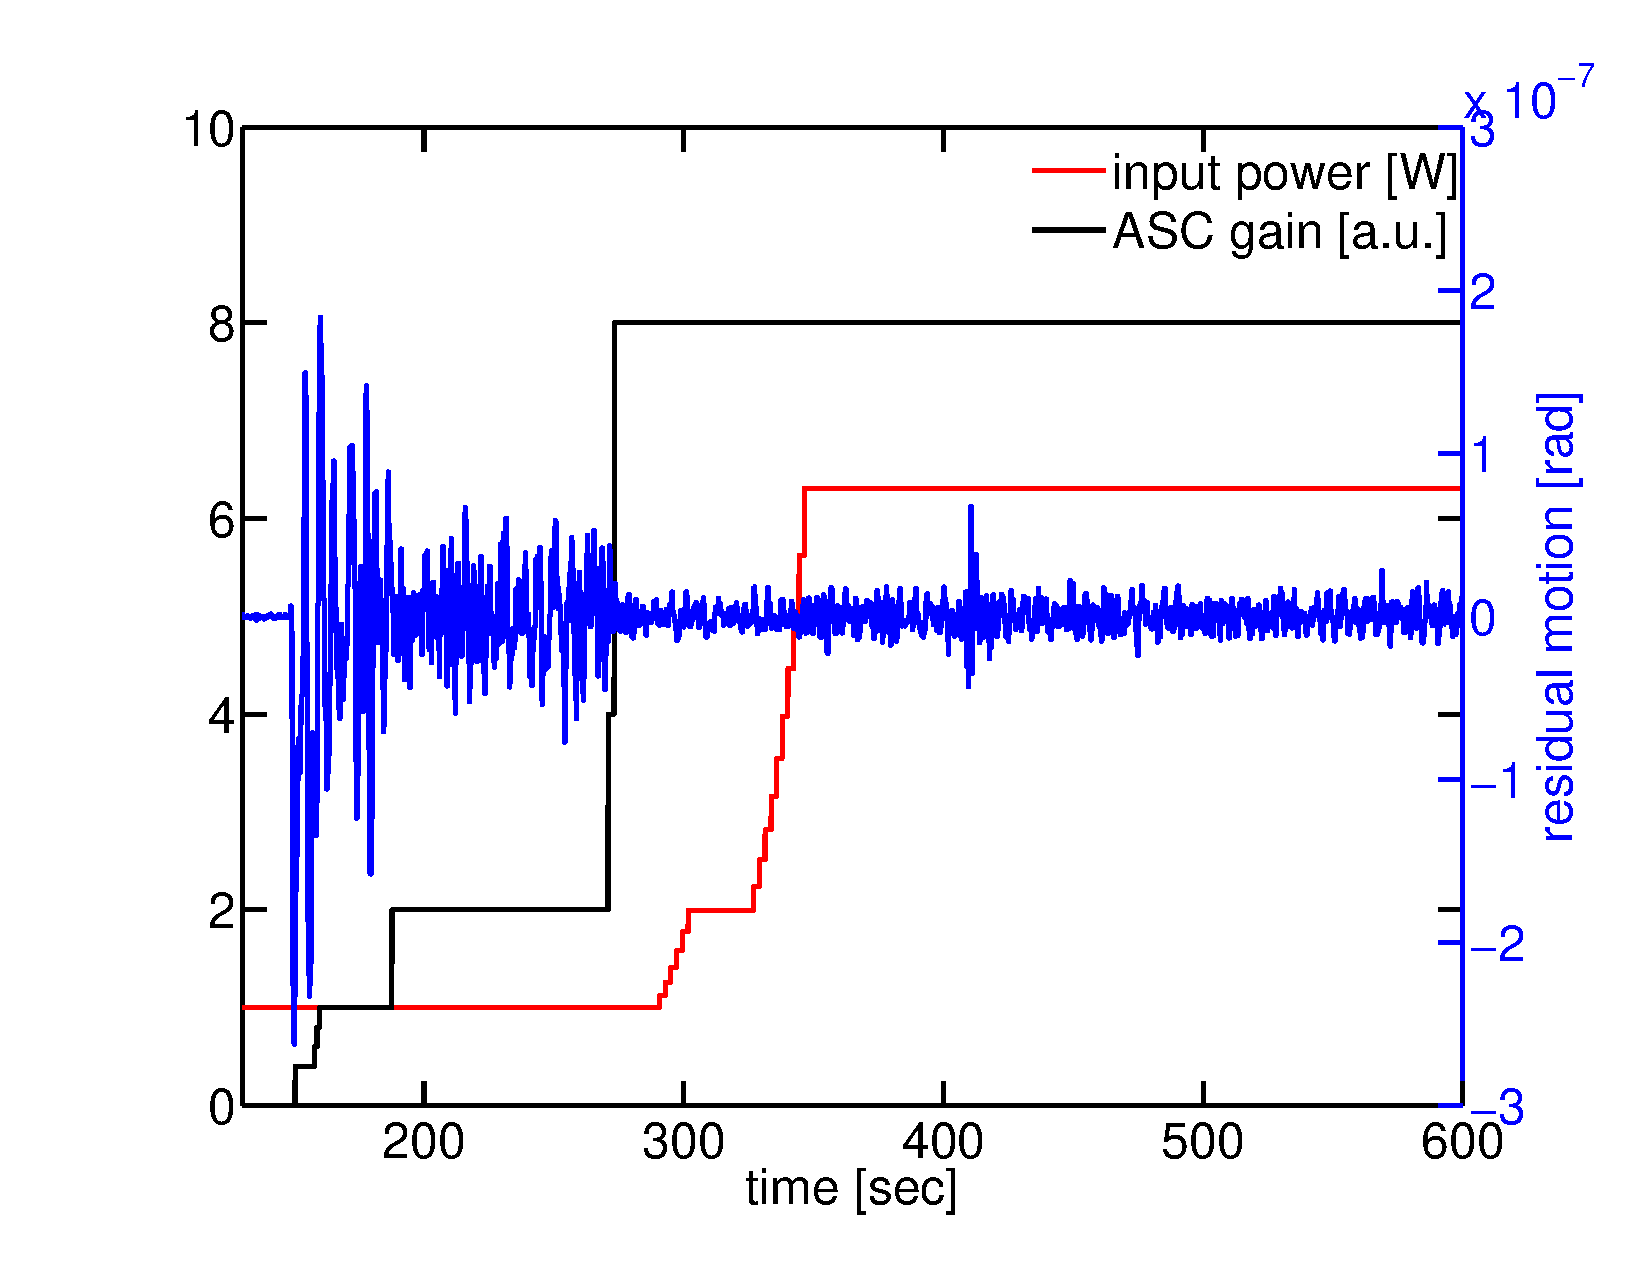
\includegraphics[width=0.7\textwidth]{figures/wfs1p_onoff.pdf}
\caption{Differential unstable residual cavity motion as the ASC gain
  is ramped up.}
\label{fig:wfs1_onoff}
\end{centering}
\end{figure}

\section{Open loop gains and opto-mechanical TFs}
\begin{itemize}
\item explain measurement
\item show plots
\end{itemize}

\section{Heating related measurements}
\begin{itemize} 
\item effect of PRC g-parameter on ASC sensing matrix
\item SPOB power scaling
\end{itemize}

\section{DC readout related measurements}
\begin{itemize}
\item RF created from DC offset beam moving on WFS1
\item RF vs DC vs power comparison of (AS) beam spot motion on WFS1
\end{itemize}

\section{ASC noisebudget}
\begin{itemize}
\item seismic - breakdown of soure of motion
\item L2A
\item input beam 
\item electronics noise
\item shot noise
\end{itemize}

\section{ASC to DARM noisebudget}
\begin{itemize} 
\item describe ASC/optical lever measurement
\item show results
\item input beam motion to DARM
\end{itemize}

The cut-off frequency of the lowpass filters for the WFS control are
of particular importance in the DARM noisebudget. The lowpass filter
is necessary for suppressing the impression of sensing noise on
suspension control. 

\begin{figure}
\begin{centering}
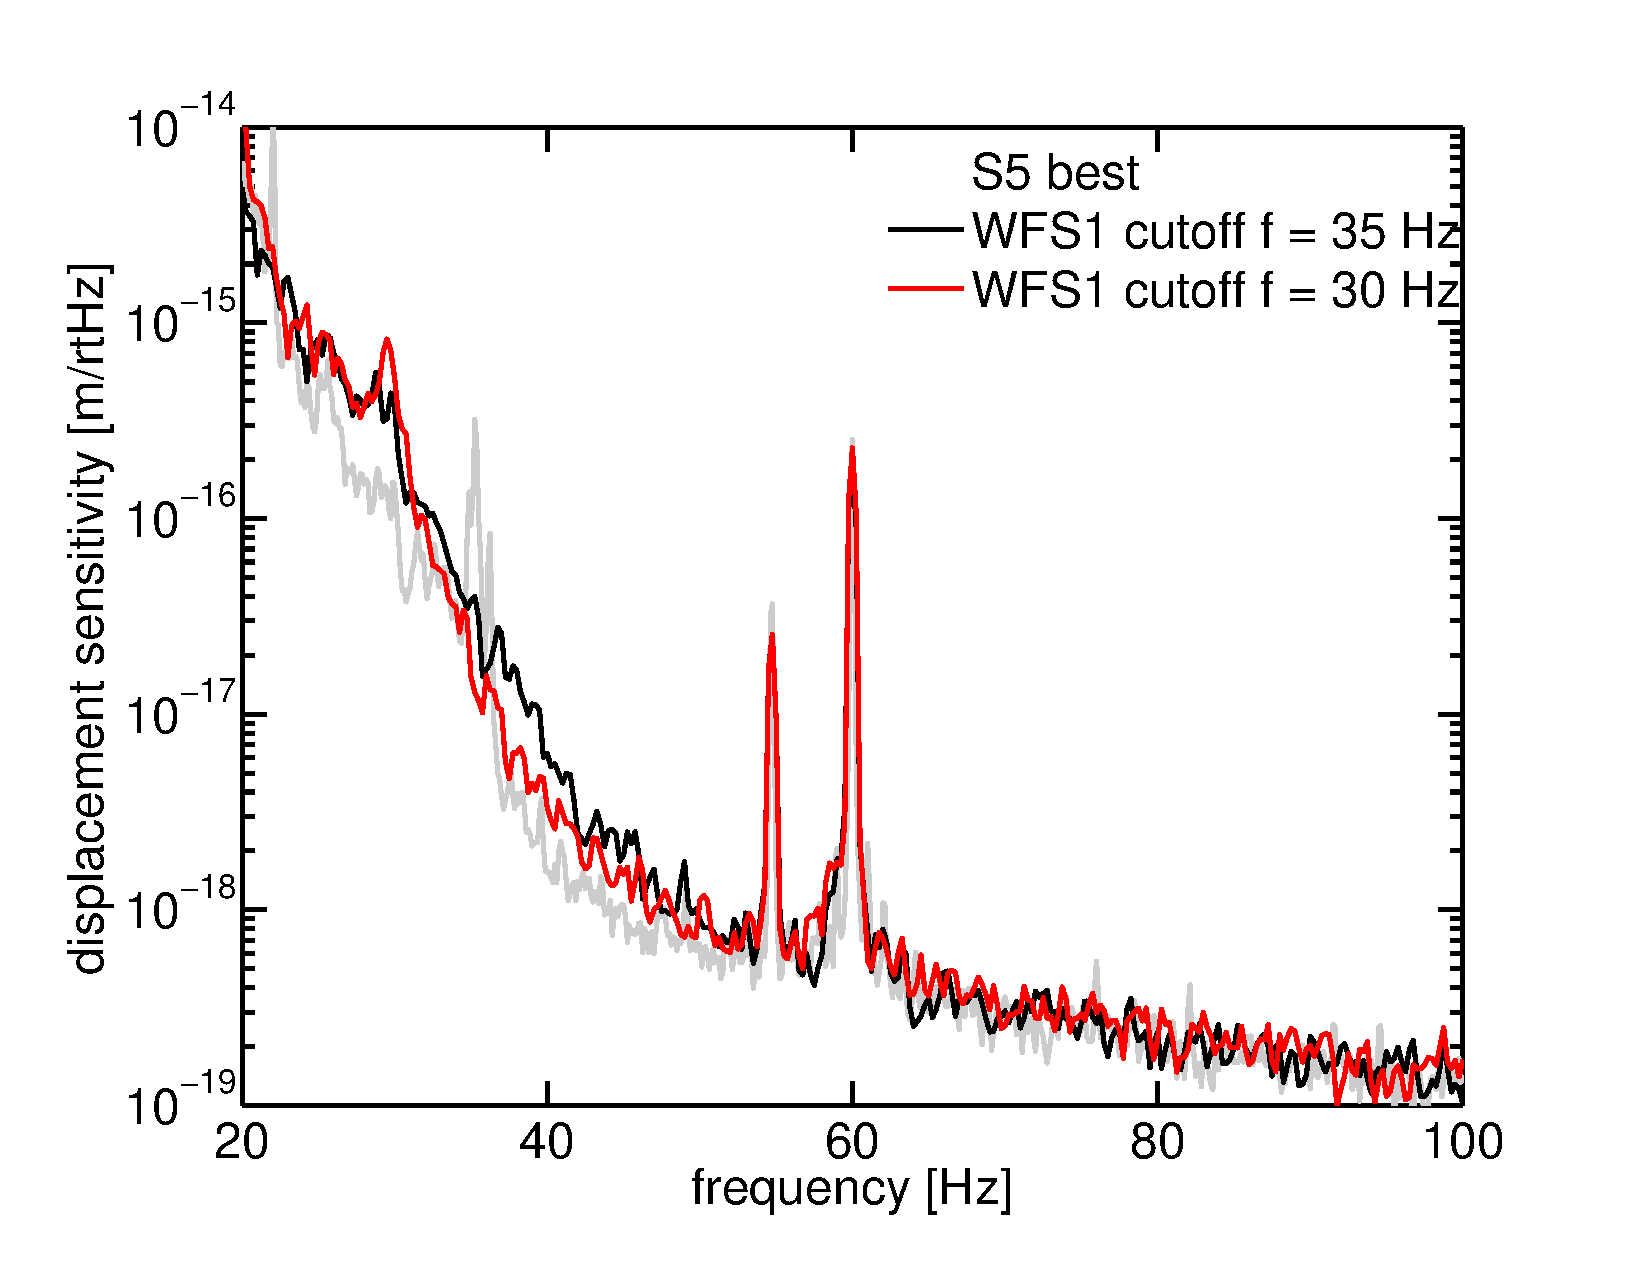
\includegraphics[width=0.8\textwidth]{figures/cutoffWFS1_DARM.pdf}
\caption{Effect of the WFS1 lowpass filter cutoff frequency on strain sensitivity.}
\label{fig:WFS1cutoff}
\end{centering}
\end{figure}


